\documentclass[../main.tex]{subfiles}

\begin{document}

\subsection{Solution overview}

The proposed solution consists of two main sections: a drone and a control section. The user will import
the mobility pattern and the constraints to the control section, which is a laptop. Then the user will send high-level commands to the drone agent, which will apply certain operations such as start/stop etc. Once the user finishes importing the mobility pattern and starting the drone mission, the drone will begin to take off and begin to visit the area to scan for getting the most number of mobile targets using \gls{drl} model. Users will keep receiving live updates and the status of service on the control section using Wi-Fi. Most of the connections in the system are wireless, which will have benefits and drawbacks.


\subsection{High level architecture}
Figure 1 shows a high-level architecture of a complete working system, in which a group of connected tools and devices are combined into a single system.In the next section, hardware and software details will be presented in a more detailed way
\begin{figure}[H]
	\centering
	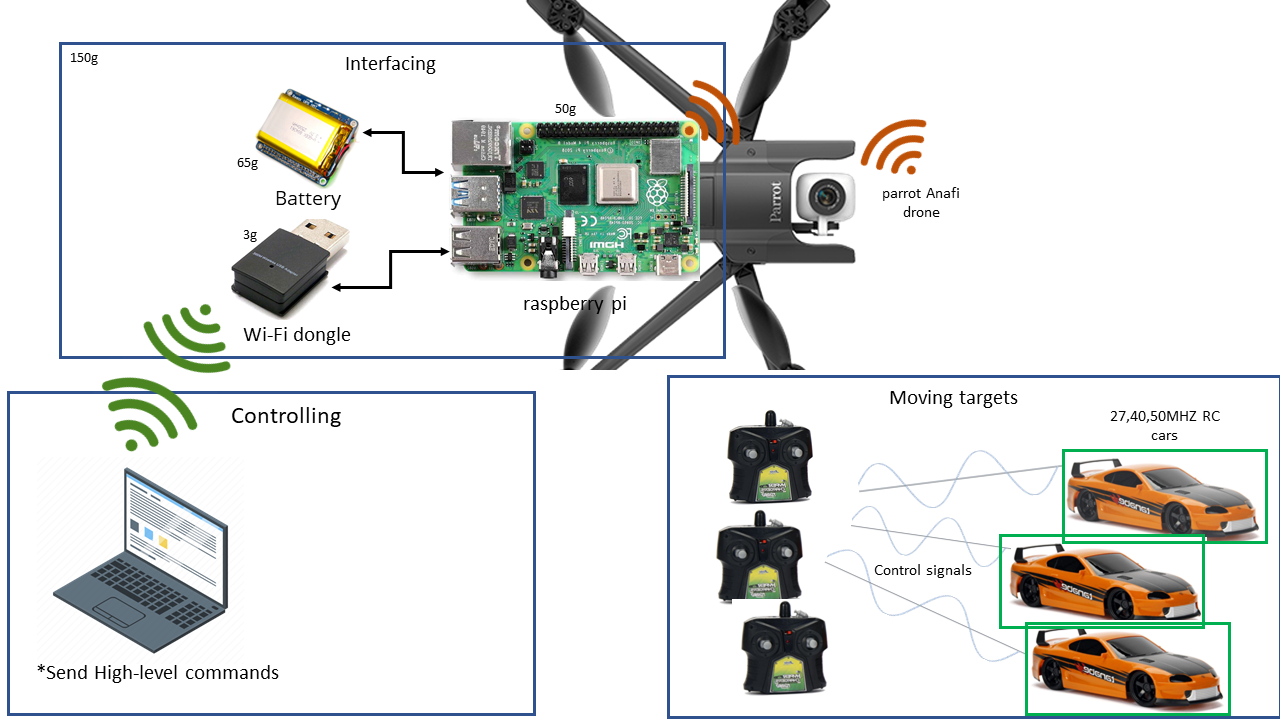
\includegraphics[width=0.9\textwidth]{high-level-arch.png}
	\caption{High-Level Architecture}\label{fig1:arch-fig}
\end{figure}


\subsection{Hardware/software to be used}

\subsubsection{Software}
%parrot olympe
%parrot sphinx
%Gazebo simulator
%roboflow
%google colab notebook /jupyter notebook
The software section contains three primary parts simulation, training, and application. The first part will focus on simulating the environment, testing the models, and flight control. Before discussing the software to be used, we will use the operating system, the base for our software applications. We selected Ubuntu 18.04 operating system for several reasons. One key reason is the compatibility because parrot Olympe and shpinx are only supported on limited distributions and operating systems. Another reason its a lite os and can be installed on the onboard computer that will be attached to the drone.For the simulation part, using shpinx and gazebo software is very helpful in visualizing the environment and how drone flight and apply the model.[more talk about simulation].In the training part, we used the simulation tools to generate some training datasets. We use a website called roboflow which helped us label the objects and generate new datasets from the existing dataset with modified constraints. For the object detection model, google colab notebook was a suffient tool to start training using \gls{cnn} Yolov5.[more talk about roboflow/training].Application software used in this project was parrot Olympe to send commands to the drone and control the flight trip and how the drone moves.[more talk about application software].


\subsubsection{Hardware}
%Parrot ANAFI Drone
%Raspberry Pi 4
%lithium Battery
%Wi-Fi adapter dongle
%laptop control station
The main core of the hardware part is the drone which in our work will be Parrot ANAFI drone. This one got couple of features that made us choosing it.[] 

\end{document}
